\setchapterimage[6cm]{seaside}
\setchapterpreamble[u]{\margintoc}
\chapter{Introduction en Français}
\labch{intro_french}

\section{L'égalité dans la Théorie des Types Intensionnelle}

Si vous avez déjà utilisé un assistant de preuve basé sur la théorie des types 
intensionnelle comme \Coq, \Agda ou \Lean -- et il y a de fortes chances que 
ce soit votre cas si vous êtes en train de lire cette thèse -- alors vous savez 
sans doute que l'égalité peut être un véritable casse-tête.

D'une part, nous avons l'égalité définitionnelle (également appelée conversion), 
qui enregistre les équations que l'assistant de preuve manipule silencieusement 
pour nous. 
% 
\sideremark{Dans un assistant de preuve basé sur la théorie des ensembles ZF 
  comme Metamath, le théorème \( {2+2=4} \) demande une preuve. 
  Et bien qu'elle soit élémentaire, cette preuve implique une quantité surprenante 
  de lemmes auxiliaires !}
% 
Par exemple, les termes \( 2 + 2 \) et \( 4 \) sont égaux défintionnellement, 
ce qui signifie que nous pouvons les utiliser indifféremment dans nos preuves 
sans avoir à nous soucier de prouver leur égalité à la main. 
% 
Lorsqu'on utilise des types dépendants, cette quantité minimale 
d'automatisation est absolument vitale ; pour éviter de se retrouver à insérer 
des coercitions explicites à chaque fois que nous voulons, par exemple, 
utiliser un terme de type \( \mathsf{Vector}\ (2+2) \) en tant que terme de 
type \( \mathsf{Vector}\ 4 \).

Mais malheureusement, il existe des objets qui ne sont pas des entiers 
naturels\sidenote{[référence nécessaire]}, et les preuves mathématiques traitent 
souvent d'égalités entre des objets infinitaires tels que les fonctions et les 
ensembles. 
% 
Et naturellement, il n'existe pas d'algorithme capable de décider si deux 
fonctions de type \( \Nat \to \Nat \) associent les mêmes images aux mêmes 
antécédants.
% 
Ainsi en pratique, l'égalité définitionnelle se limite aux égalités 
\( \beta / \eta / \iota \), avec possiblement quelques extensions comme les 
règles de réécriture d'Agda~\sidecite{taming_of_the_rew}.

Puisque le système ne sera pas en mesure d'automatiser complètement toutes 
les égalités, nous avons besoin d'un moyen de raisonner à leur sujet. 
% 
C'est pourquoi la théorie des types intensionnelle fournit une deuxième notion 
d'égalité, appelée l'égalité \emph{propositionnelle}.
% 
Contrairement à l'égalité définitionnelle, celle-ci est disponible 
dans le langage de la théorie des types, et nous pouvons l'utiliser 
pour énoncer et prouver des théorèmes. 
% 
Dans les trois principaux assistants de preuve basés sur la théorie des types, 
l'égalité propositionnelle est implémentée avec un type inductif, d'après les 
travaux de Martin-Löf~\sidecite{MartinLoef75}.
% 
\sideremark{L'égalité propositionnelle \( \Indeq{A}{t}{u} \) est un type, tandis
  que l'égalité définitionnelle \( \eqtm{\Gamma}{t}{u}{A} \) est un jugement de typage.}
\begin{mathpar}
  \inferrule{\tyty{\Gamma}{A}
			\\ \tytm{\Gamma}{t}{A}
			\\ \tytm{\Gamma}{u}{A}}
			{\tyty{\Gamma}{\Indeq{A}{t}{u}}}
  \and
  \inferrule{\tyty{\Gamma}{A}
			\\ \tytm{\Gamma}{t}{A}}
			{\tytm{\Gamma}{\indrefl{t}}{\Indeq{A}{t}{t}}}
\end{mathpar}
\begin{mathpar}
  \inferrule{\tyty{\Gamma}{A}
			\\ \tytm{\Gamma}{t}{A}
			\\ \tytm{\Gamma}{B}{\Depfun{A}{\Fun{t =_A x}{\Univ}}}
			\\ \tytm{\Gamma}{u}{B\ t\ \mathsf{refl}_t}
			\\ \tytm{\Gamma}{t'}{A}
			\\ \tytm{\Gamma}{e}{t =_A t'}}
			{\tytm{\Gamma}{\mathsf{J}(A,t,B,u,t',e)}{B\ t'\ e}}
\end{mathpar}
\begin{mathpar}
  \inferrule{[...]}
			{\red{\Gamma}{\mathsf{J}(A,t,B,u,t,\mathsf{refl}_t)}{u}{B\ t\ \mathsf{refl}_t}}
\end{mathpar}

Ces quelques règles suffisent à définir une relation d'équivalence qui contient 
l'égalité définitionnelle, peut être utilisée pour réécrire des termes et peut 
être utilisée pour convertir des termes entre deux types égaux.

Une différence importante avec la pratique courante des mathématiques est que nous restons 
très attachés à la correspondance de Curry-Howard entre les preuves et les programmes : 
l'égalité est un type, et les preuves d'égalité sont des programmes\sidenote{amen.}. 
% 
En tant que telles, les preuves d'égalité sont des valeurs de première classe 
tout comme les entiers naturels ou les fonctions, et elles sont donc sujettes 
au raisonnement mathématique, et elles peuvent également être évaluées.

\subsection{Types et Propositions}

Bien que la possibilité d'évaluer les preuves soit un principe fondamental de 
la philosophie Curry-Howard, une preuve d'égalité typique n'a pas un 
comportement calculatoire très intéressant. 
% 
Le terme \( \indJ{A}{t}{P}{u}{t'}{e} \) se contente d'attendre que \( e \) se 
réduise en une preuve par réflexivité, auquel cas \( t \) et \( t' \) sont 
convertibles et le terme entier peut simplement être évalué en \( u \).

Par conséquent, les programmes 
\defnote{extraits}{L'extraction produit un programme dans un langage externe
  en effaçant une partie des types.} 
à partir de preuves qui utilisent du raisonnement équationnel ont tendance à 
passer beaucoup de temps à propager les preuves d'égalité, pour finir par les 
effacer lorsqu'elles ne sont plus nécessaires. 
% 
Cette situation sous-optimale a conduit l'assistant de preuve de Coq à 
introduire une sorte spéciale \( \varProp \) pour les types dont les preuves sont 
effacées lors de l'extraction~\sidecite{letouzey04}. 
% 
En plaçant l'égalité propositionnelle dans \( \varProp \) avec les autres 
contraintes logiques qui ne jouent aucun rôle calculatoire, Coq retrouve des 
performances raisonnables pour les programmes extraits.

Techniquement, c'est un peu une violation de la discipline de Curry-Howard, 
puisque \( \varProp \) réintroduit une séparation entre les propositions et les données.
%  
Mais ne vous méprenez pas : les preuves de propositions jouent encore
leur rôle normal dans les calculs de théorie des types, et en particulier, 
elles peuvent bloquer l'évaluation des termes ouverts. 
% 
C'est seulement lorsque nous extrayons un programme \emph{externe} que les 
propositions sont effacées.

L'assistant de preuve \Lean va un peu plus loin et introduit la sorte 
\( \varsProp \) pour les \emph{propositions strictes}~\sidecite{lean}. 
% 
Contrairement aux propositions de \Coq, les propositions strictes sont
\emph{proof-irrelevant}, ce qui signifie que deux habitants quelconques 
d'une proposition stricte \( A \) sont définitionnellement égaux.
% 
\[
\inferrule{\tytm{\Gamma}{A}{\varsProp} \\ \tytm{\Gamma}{t, u}{A}}{\eqtm{\Gamma}{t}{u}{A}}
\]

Mettre l'égalité propositionnelle dans \( \varsProp \) n'est pas aussi inoffensif 
qu'il n'y parait.
% 
En particulier, cela implique que toute preuve d'égalité propositionnelle entre 
deux termes convertibles est maintenant indiscernable d'une preuve par réflexivité 
(puisque les deux preuves ont le même type). 
% 
En d'autres termes, \Lean satisfait une version stricte du principe de 
\emph{uniqueness of identity proofs} (UIP).

Avec ce principe, les preuves d'égalité non-réflexives ne sont plus capables de 
bloquer un calcul : le terme \( \indJ{A}{t}{P}{u}{t}{e} \) est convertible en 
\( \indJ{A}{t}{P}{u}{t}{\indrefl{t}} \), qui devrait se réduire !
% 
Par conséquent, l'éliminateur \( J \) de \Lean se réduit dès qu'il est appliqué 
à deux termes définitionnellement égaux.
\begin{mathpar}
  \inferrule[J-conv]{[...] \\ \eqtm{\Gamma}{t}{t'}{A}}
			{\red{\Gamma}{\mathsf{J}(A,t,B,u,t',e)}{u}{B\ t'\ e}}
      \ilabel{infrule:J-conv}
\end{mathpar}

Mais bien que cette règle soit logiquement cohérente, Abel et Coquand ont montré 
qu'elle conduit à un échec de la normalisation pour les termes 
ouverts~\cite{lmcs:6606}. 
% 
\sideremark{Il est établi que l'égalité définitionnelle de \Lean est indécidable
  pour des raisons orthogonales~\cite{gilbert:hal-01859964}. Toutefois, 
  remarquons que ça n'a pas empêché la communauté de \Lean de développer 
  une impressionante quantité de mathématiques.}
% 
Et comme les algorithmes que nous utilisons pour vérifier la convertibilité 
reposent sur la normalisation, on en déduit que l'ajout de la 
règle~\nameref{infrule:J-conv} casse notre procédure de décision pour l'égalité 
définitionnelle. 
% 
Comme l'ont remarqué Abel et Coquand, il n'est pas clair que cela provienne d'une 
incompatibilité fondamentale entre les propositions strictes imprédicatives et 
l'égalité propositionnelle, et qu'il n'existe pas une stratégie plus 
intelligente qui pourrait résoudre ce problème.

\subsection{Imprédicativité}

En théorie des types dépendants, une sorte est qualifiée d'\emph{imprédicative} 
lorsqu'elle est close par produits dépendants indexés par n'importe quel type. 
% 
Par exemple la sorte des propositions de \Coq est imprédicative, car pour tout 
type \( A \) et toute fonction \( \tm{B}{A \to \varProp} \) le produit dépendant 
\( \Depfun{A}{B\ x} \) est dans \( \varProp \).

L'imprédicativité introduit de l'autoréférence dans notre système 
de types : nous pouvons l'utiliser pour former une proposition \( P \) qui 
quantifie sur le type \( \varProp \) de toutes les propositions, type qui 
contient \( P \). 
% 
Un exemple classique est l'encodage imprédicatif de la proposition fausse, 
dont les habitants peuvent être éliminés dans n'importe quelle autre proposition :
\[
\Depfun[X]{\varProp}{X} \quad : \quad \varProp
\]

Comparez cette situation avec la hiérarchie \emph{prédicative} 
$(\varType_i)_{i \in \Nat}$ 
% 
\sideremark{Dans l'assistant de preuve \Coq, les univers prédicatifs ne sont 
  techniquement pas indexés par des entiers, mais le système maintient un graphe
  de contrainte de niveau d'univers qui remplit la même fonction.}
% 
des types non-propositionnels.
% 
Dans le monde non-propositionnel, les produits dépendants sont forcés de vivre 
dans un niveau d'univers qui est à la fois plus grand que celui de leur domaine et
plus grand que celui de leur codomaine :
% 
étant donné un type \( A : \varType_i \) et une fonction \( {\tm{B}{A \to \varType_j}} \), 
le produit dépendant \( \Depfun{A}{B\ x} \) atterrit dans l'univers
\( \varType_{\mathsf{max}(i,j)} \).
 
La prédicativité supprime les possibilités d'autoréférence : si nous essayons 
de reproduire l'encodage de la proposition fausse dans \( \varType_0 \), le 
type résultant se retrouve dans l'univers \( \varType_1 \).
\[
\Depfun[X]{\varType_0}{X} \quad : \quad \varType_1
\]

Autoriser l'autoréférence revient à jouer avec le feu : les antinomies 
logiques héritées du paradoxe de Russell restent tapies dans l'ombre, et 
pourraient nous attraper si nous sommes un peu trop gourmands avec nos 
règles logiques.
% 
Par exemple, le paradoxe de Berardi montre qu'avoir le tiers exclu et les 
l'élimination large pour les booléens à valeur dans \( \varProp \) est incohérent. 
% 
L'imprédicativité joue également un rôle central dans le terme 
non-normalisant qu'Abel et Coquand ont obtenu à partir de la 
règle~\nameref{infrule:J-conv}~\sidecite{lmcs:6606}.

En contrepartie pour cette fragilité, l'imprédicativité augmente considérablement 
le pouvoir expressif de notre système logique, et nous permet de formuler 
d'importantes constructions mathématiques telles que le théorème du point fixe 
de Tarski ou des treillis complets non-triviaux~\sidecite{paco}. 
% 
De plus, certains théorèmes comme la normalisation du Système F ne peuvent tout
simplement pas être prouvés dans une théorie prédictive.

Les différents assistants de preuve ont adopté des attitudes variées envers 
l'imprédicativité. D'un côté, 
% 
\sideremark{Fut un temps, \Coq utilisait également une sorte imprédicative
  pour les types \emph{proof-relevant}, mais l'équipe de développement a 
  préféré désactiver cette fonctionnalité pour avoir une théorie plus proche
  des mathématiques classiques.}
% 
\Coq et \Lean ont tous deux adopté l'imprédicativité pour leur sorte des 
propositions, qui cohabite avec la hiérarchie d'univers prédicatifs utilisée 
pour les types \emph{proof-relevant}~\sidecite{Coq:manual,lean}.
% 
De l'autre côté, l'assistant de preuve \Agda a choisi de ne pas implémenter
l'imprédicativité et utilise deux hiérarchies prédicatives à la place, une 
pour les propositions strictes et une pour les types~\sidecite{agda261}.

\section{L'Extensionalité dans la Théorie des Types Intensionnelle}

The basic propositional equality that we defined as an inductive type does 
not quite meet the standards of mathematical reasoning.
% 
In mathematics, two functions are considered equal when they agree on all 
inputs -- this is the principle of \emph{function extensionality} --
% 
\sideremark{In particular, it is not possible to prove that the functions
\( {\lambda\ n\ .\ n+1} \) and \( {\lambda\ n\ .\ 1+n} \) are equal.}
% 
but this principle is not derivable for the propositional equality in 
intensional type theory.
\[
  \Indeq{A \to B}{f}{g} \quad \xcancel{\longleftrightarrow} \quad \Depfun{A}{\Indeq{B}{f\ x}{g\ x}}
\]

In fact, we can show that all proofs of propositional equality in an empty 
context reduce to the definitional equality.
% 
This is a straightforward consequence of the normalization of well-typed terms:
the sole closed normal form for an equality proof is \( \indrefl{t} \), which
only type-checks if the two endpoints are convertible.
% 
And as we explained earlier, the definitional equality does not handle pointwise
equality of functions.

% All in all, the propositional equality is better thought of as an equality 
% between programs than as an equality between mathematical objects.

Developing sophisticated mathematics without the principle of 
function extensionality is not an easy task.
Consequently, the community has explored several options to recover a more 
conventional equality throughout the years.

\paragraph*{Extensionality axioms}
% 
The most obvious way to recover a missing reasoning principle is simply to
postulate it as an axiom. 
% 
\sideremark{Note that in \Coq and \Lean it is still possible to extract a program 
  from a proof that postulates function extensionality, because the axiom
  is erased during extraction.}
% 
For instance, the axiom \textsf{functional\_extensionality\_dep} is available 
in \Coq's standard library.
% 
The downside of using axioms is that they do not play so well with the 
computational properties of intensional type theory:
% 
% intensional type theory is built around the proofs-as-programs correspondence, 
% and every existence proof doubles as an algorithm that computes the witness
% of existence.
% 
applying the \( J \) eliminator to an equality obtained \textit{via} an axiom
will only result in a stuck term.

\paragraph*{Setoids}
% 
A standard technique to recover extensionality principles without breaking the
proofs-as-programs correspondance is to use \emph{setoids}~\sidecite{hofmann95},
\ie to replace types with pairs \( (|A|, e_A) \) of a carrier type \( |A| \)
and an equivalence relation \( e_A \) on \( |A| \) 
(the \emph{setoid equality} of \( A \)).
% 
We then restrict our attention to functions that preserve the setoid equality, 
and we bake function extensionality into the setoid equality of function types.

Working with setoids is not exactly pleasant, as we need to supplement every
definition with bureaucratic proofs of preservation of the setoid equalities,
even though all available constructs in type theory do respect function 
extensionality~\sidecite{Altenkirch99}.
% 
Basically, we need to do the work of a compiler by hand.
% 
The \Coq proof assistant provides some automation to deal with setoids through 
tactics, but these solutions do not scale painlessly to large developments -- 
to the point that the community has coined the term \emph{setoid hell} to refer 
to these issues.

\paragraph*{Alternative type theories}
% 
Since extensionality axioms are problematic because they block 
computation, type theorists have explored numerous ways to extend intensional
type theory with new computational rules that handle the desired axioms.
% 
The most successful lines of work can be roughly divided into two groups: the 
ones that replace the inductive propositional equality with an \emph{observational equality}, 
and the ones that replace it with a \emph{univalent equality}.
% 
% In the first half of this thesis, we will restrict our attention to the first 
% group. The univalent equality is at the center of the second half, and we 
% invite the interested reader to have a look at \cref{ch:hott}.

\subsection{Observational Equality}

The observational equality has its roots in the work of Hofmann and 
Altenkirch on the setoid model of type theory~\cite{hofmann95,altenkirch99}.
% 
By interpreting types as setoids, they were able to model
\defnote{ITT+funext}{ITT+funext stands for intensional type theory extended 
  with function extensionality.}
in an intensional type theory extended with strict propositions.
% 
Since these strict propositions do not conflict with the proofs-as-programs 
interpretation, the setoid model provides a way to evaluate proofs that use a 
function extensionality axiom by evaluating their interpretation.

The central ingredient of the setoid model is the interpretation of the 
universe.
% 
Constructing a setoid of small setoids seemed difficult at first, because 
the collection of all small setoids does not have a natural setoid equality;
but this can be solved by using an 
\defnote{inductive-recursive}{Induction-recursion is a powerful principle that 
  allows us to define an inductive type \( A \) simultaneously with functions
  defined by recursion on \( A \).}
universe of codes on which the setoid equality and type coercion operators are 
defined by recursion.

Following this first step, Altenkirch McBride and 
Swierstra~\sidecite{altenkirchAl:plpv2007} developed observational 
type theory (OTT), an extension of intensional type theory that brings the main 
insights of the setoid model back to the world of syntax:
% 
OTT introduces a new primitive operator called the \emph{observational equality} that 
equips every type with a setoid structure defined by recursion on the universe.
% 
The result is a type theory that supports the principles of UIP and function 
extensionality, and Altenkirch \etal prove that normalization of OTT terms 
follows from a conjectured normalization result for type theory with 
induction-recursion.

The observational equality has seen some new and exciting developments in recent 
years, such as the work of Sterling \etal who revisit it under the lens of 
cubical type theory~\sidecite{sterling-angiuli-gratzer:2022} or the setoid
type theory of Altenkirch \etal~\sidecite{Altenkirch2019}.
% 
Still, observational type theory has yet to reach a level of maturity 
comparable to that of univalent type theories.
% 
In particular, there is still no support for the observational equality in
major proof assistants, despite some valiant efforts~\sidecite{mcbride-autopsy}.

\subsection{Univalent Equality}

The other line of work is more recent and takes its roots in
Voevodsky's \emph{univalence axiom}~\sidecite{kapulkin2012simplicial,hottbook}.
\[
(A =_{\varType} B) \enskip \simeq \enskip  (A \simeq B)
\]
The univalence axiom gives a new meaning to the equality between types: 
% 
\sideremark{The correct definition of an isomorphism between types is somewhat 
  subtle, so we will simply take it as granted for the time being.}
% 
a witness of equality between \( A \) and \( B \) is now the same as an element of the type 
\( A \simeq B \) of \emph{isomorphisms} between \( A \) and \( B \). 
% 
This can be seen as an extensionality principle for the universe of types, and
adding it to intensional type theory has far reaching consequences. 
In particular, univalience implies the principle of function extensionality.

\paragraph*{Homotopy Type Theory}
% 
The univalence axiom departs from the standard mathematical usage of equality, 
in that equality can no longer be a proposition since it now contains essential
computational information. 
% 
For instance there are two distinct automorphisms of the type of booleans 
-- one corresponding to the identity and the other to negation -- and transporting along
the identity is not the same as transporting along negation.
\sideremark{Transporting along an isomorphism amounts to an application of the
  isomorphism, up to a propositional equality.}
\[
\begin{split}
\indJ{\varType}{\mathsf{Bool}}{\lambda X\ .\ X}{\mathsf{true}}{\mathsf{Bool}}{\mathsf{id}} & \enskip =_{\mathsf{Bool}} \enskip \mathsf{true} \\
\indJ{\varType}{\mathsf{Bool}}{\lambda X\ .\ X}{\mathsf{true}}{\mathsf{Bool}}{\mathsf{neg}} & \enskip =_{\mathsf{Bool}} \enskip \mathsf{false}
\end{split}
\]

Thus when we use the univalence axiom, we must accept that types now contain 
important information in their equality types. 
% 
But these equality types also contain information in their own equality types,
and so on. 
% 
We end up with infinite towers of relevant equality types, all contained in the
data of a type.

\begin{figure}[!h]
  \tikzset{every picture/.style={line width=0.75pt}} %set default line width to 0.75pt        
  \begin{minipage}{0.4\textwidth}
    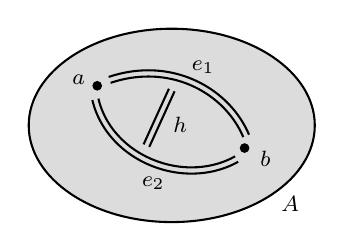
\begin{tikzpicture}[x=0.75pt,y=0.75pt,yscale=-1,xscale=1,roundnode/.style={circle, fill=black, inner sep=0pt, minimum size=3.5pt}]
    %uncomment if require: \path (0,300); %set diagram left start at 0, and has height of 300

    %Shape: Ellipse [id:dp3643970014729053] 
    \draw  [fill={rgb, 255:red, 220; green, 220; blue, 220 }  ,fill opacity=1 ] (4,52.08) .. controls (4,26.36) and (34.86,5.5) .. (72.92,5.5) .. controls (110.98,5.5) and (141.83,26.36) .. (141.83,52.08) .. controls (141.83,77.81) and (110.98,98.67) .. (72.92,98.67) .. controls (34.86,98.67) and (4,77.81) .. (4,52.08) -- cycle ;
    %Curve Lines [id:da06896022650610556] 
    \draw    (42.51,28.73) .. controls (49.06,26.53) and (55.48,25.53) .. (61.61,25.53) .. controls (81.63,25.53) and (98.59,36.2) .. (107.29,50.91) .. controls (108.37,52.74) and (109.33,54.63) .. (110.14,56.57)(43.46,31.57) .. controls (49.69,29.48) and (55.78,28.53) .. (61.61,28.53) .. controls (80.48,28.53) and (96.5,38.56) .. (104.71,52.44) .. controls (105.72,54.15) and (106.61,55.92) .. (107.38,57.73) ;
    %Curve Lines [id:da08140854638152761] 
    \draw    (37.58,39.19) .. controls (41.3,54.8) and (53.94,65.9) .. (68.57,70.27) .. controls (72.96,71.58) and (77.53,72.28) .. (82.1,72.31) .. controls (82.22,72.31) and (82.34,72.31) .. (82.46,72.31) .. controls (89.71,72.31) and (96.96,70.63) .. (103.45,66.99)(34.66,39.89) .. controls (38.64,56.55) and (52.07,68.48) .. (67.72,73.14) .. controls (72.37,74.53) and (77.23,75.28) .. (82.08,75.31) .. controls (82.2,75.31) and (82.33,75.31) .. (82.46,75.31) .. controls (90.22,75.31) and (97.97,73.5) .. (104.92,69.61) ;
    %Straight Lines [id:da7856762818241472] 
    \draw    (74.28,35.66) -- (62.08,62.46)(71.55,34.42) -- (59.35,61.22) ;

    \node[roundnode] (B0) at (37,33) {};
    \node (C0) at (28,30) {\footnotesize{$a$}};
    \node[roundnode] (B1) at (108,63) {};
    \node (C1) at (118,68) {\footnotesize{$b$}};
    \node (C2) at (88,24) {\footnotesize{$e_1$}};
    \node (C3) at (64,80) {\footnotesize{$e_2$}};
    \node (C4) at (77,52) {\footnotesize{$h$}};
    \node (C5) at (130,90) {\footnotesize{$A$}};
    \end{tikzpicture}
  \end{minipage}
  \begin{minipage}{0.4\textwidth}
  \[
    \begin{array}{l}
      A : \varType_i \\
      a : A \\
      b : A \\
      e_1 : \Indeq{A}{a}{b} \\
      e_2 : \Indeq{A}{a}{b} \\
      h : \Indeq{(\Indeq{A}{a}{b})}{e_1}{e_2}
    \end{array}
  \]
  \end{minipage}
  \caption{Graphical representation of a type with inhabitants and equalities}
\end{figure}
 
All in all, these types do not really resemble sets anymore. 
% 
Voevodsky noticed that they are much closer to \emph{weak \( \infty \)-groupoids}, 
a higher categorical gadget that plays an important role in homotopy theory, 
the branch of math that studies spaces and their deformations.
% 
This is the starting point of \emph{homotopy type theory} (HoTT), a far-reaching analogy
between homotopy theory and intensional type theory with the univalence 
axiom~\cite{hottbook}.

In homotopy theory, we think of types as spaces. Inhabitants of a type 
play the role of its points, equalities between two terms correspond to paths
between the points, equalities between two equalities are continuous
deformations between the corresponding paths, and so on. 
% 
Naturally, functions between types are continuous in that they preserve
equalities, and isomorphisms correspond to homotopy equivalences.

Homotopy type theory also extends the notion of inductive type to 
\emph{higher inductive types} (HITs), which feature constructors for paths/equalities
in addition to constructors for elements.
% 
HITs provide a variety of basic spaces, such as the circle, the sphere and
the torus, but also a notion of quotient types.
% 
\sideremark{This definition of the \textsf{circle} type might be surprising,
  as it looks nothing like the expected space
  \( \{ (x, y) \in \mathbb{R}^2\ |\ x^2 + y^2 = 1 \} \).
  This is because types in HoTT are not \emph{topological} spaces, but rather
  synthetic spaces built out of points, paths and higher dimensional faces.
  As such, the \textsf{circle} is freely generated by a base point and a path
  from that base point to itself.}
\[
\begin{array}{l}
\mathsf{Inductive}\enskip\mathsf{circle} : \varType_0\enskip := \\
\sep \quad \mathsf{base} \enskip : \enskip \mathsf{circle}\\
\sep \quad \mathsf{loop} \enskip : \enskip \Indeq{\mathsf{circle}}{\mathsf{base}}{\mathsf{base}} \\
\\
\mathsf{Inductive}\enskip\mathsf{quotient}\ (A : \varType_i)\ (R : A \to A \to \varType_i) : \varType_i\enskip := \\
\sep \quad \mathsf{emb} \enskip : \enskip A \to \mathsf{quotient}\ A\ R \\
\sep \quad \mathsf{quo} \enskip : \enskip \Depfun[a\ b]{A}{R\ a\ b \to \Indeq{...}{\mathsf{emb}\ a}{\mathsf{emb}\ b}} \\
\end{array}
\]

Using higher inductive types and the univalence axiom it becomes possible to 
prove a surprising amount of classical results from homotopy theory, rephrased
to talk about types and equality:
% 
in his PhD thesis, Brunerie managed to show that the fourth homotopy group of
the three-dimensional sphere has two elements~\sidecite{Brunerie16}.
% 
Since then, the HoTT community has developed extensive libraries of formalized
univalent mathematics in \Coq~\sidecite{Bauer:2017:HLF:3018610.3018615} and
\Agda~\sidecite{agda-unimath}.

However, homotopy type theory is not exactly computational. The univalence
axiom is, well, an axiom -- which means that the \( \mathsf{J} \) eliminator
will not reduce when applied to an equality that we obtained from an 
isomorphism using univalence.
% 
Higher inductive types also block computation, because their elimination 
principles are simply postulated as axioms.
% 
This situation is all the more disappointing as the features introduced by HoTT
seem to follow the principles of constructive mathematics.

\paragraph*{Cubical Type Theory}
% 
Subsequently, the type theory community directed its attention to the
search for a computational interpretation of the univalent equality. 

In 2014, Bezem Coquand and Huber built a model of the univalence axiom in a constructive 
set theory~\sidecite{BezemCoquandHuber14}.
% 
Their model interprets types as \emph{fibrant cubical sets}, a combinatorial
model of weak \( \infty \)-groupoids that lends itself well to a constructive
presentation.
% 
Although this model is not developed in type theory and does not support 
anything that resembles type theoretic computation, it paved the way for a new 
understanding of univalence.

This program came to fruition a year later with the introduction of 
\emph{cubical type theory}, an intensional type theory based on the insights 
provided by the fibrant cubical sets~\sidecite{cubicaltt}.
% 
This new system incorporates primitives from homotopy theory directly in the typing 
judgments, and provides them with adequate computation rules.
% 
With this additional structure, it becomes possible to derive the principle of 
univalence as a theorem, which makes cubical type theory an axiom-free univalent 
theory.
% 
And since it satisfies a canonicity property~\sidecite{Huber16} and supports a
normalization function for open terms~\sidecite{sterling_normalization_cubical}, 
cubical type theory can be deemed fully computational.
% 
On top of this, it supports higher inductive types with
natural elimination principles and computation rules~\sidecite{CavalloHarper19}.

In the years following its introduction, cubical type theory flourished into a 
vibrant field of research.
% 
Many variations of the original system have been studied on paper~\cite{AngiuliHouHarper18,ABCFHL}
and implemented in proof assistants~\cite{Cubicaltt, redtt}.
% 
Among them, the \texttt{cubical} mode of the \Agda proof assistant~\sidecite{cubical-agda}
is without a doubt the most successful implementation, and it has set the stage for several 
large-scale formalization projects.

% In particular, the 
% % 
% Since cubical type theory is supposed to be normalizing\sidenote{The theorem 
%   proved by Angiuli and Sterling is not } and have canonical 
% datatypes, any proof of a statement of the form \( \Depsum[n]{\Nat}{P\ n} \)
% should evaluate to a pair of an integer \( n \) and a proof of \( P\ n \).

\section{Contributions}

\paragraph{The Observational Calculus of Constructions}
% 
In the first part of this thesis, we study the meta-theoretical properties of the observational 
equality.
% 
To this end, we introduce a formal calculus based on the observational type theory
of Altenkirch \textit{et al}, which we call the Observational Calculus of Constructions, or 
\SetoidCC for short.
% 
\SetoidCC is based on dependent type theory with inductive types and an impredicative 
universe of strict propositions. 
% 
On top of this, it adds an implementation of the observational equality and a 
primitive type casting operator, from which we can derive the principles of
uniqueness of identity proofs, of function extensionality and of proposition
extensionality.
% 
\SetoidCC also supports the formation of the quotient of a type by a strict 
equivalence relation.

We equip our formal system with a reduction strategy that we use to prove a normalization 
theorem, canonicity of the basic datatypes, and decidability of the typing
relation.
% 
These results are obtained through a normalization model, that we build in \Agda using
the logical relations framework developed by Abel \etal~\sidecite{Abel:POPL2018}.
% 
The normalization proof can be browsed at \refAgdaRoot{Everything}, but links to the code
will be scattered throughout the relevant parts.

To the best of our knowledge, our model introduces several innovations compared 
to the existing literature on normalization proofs.
% 
The most basic, but also the most important one is that we do not normalize the 
proofs of strict propositions, contrary to the approach championed by 
Gilbert \etal~\sidecite{gilbert:hal-01859964}. 
% 
This allows us to not only support proof-irrelevant axioms, but also to handle 
impredicativity without resorting to the usual reducibility candidates.
% 
Without the need for reducibility candidates, we can use a proof-irrelevant
logical relation, which in turn lets us have non-parametric operators such
as the observational equality and type-casting.
% 
In counterpart for this added flexibility, normalization does not directly
imply canonicity anymore, and a separate proof of consistency of the
theory is required to derive canonicity -- as suggested by McBride \etal in
their observational type theory paper~\sidecite{AltenkirchMcBrideSwiestra07}.
% 
We bridge that gap by building a set-theoretic model for \SetoidCC.

This work solves several problems that were still open as far as we know:
% 
\sideremark{Altenkirch, McBride and Swierstra reduced normalization of 
  observational type theory to a normalization conjecture for intensional 
  type theory with induction-recursion, which has not been proven as far as we 
  know.}
% 
first and foremost, we get a proper proof of normalization and decidability for 
observational type theory, which was conjectured by Altenkirch \etal
% 
Moreover, the equality of \SetoidCC lives in an impredicative universe 
of strict propositions just like the equality of \Lean. 
% 
We show that we can interpret the \( \mathsf{J} \) eliminator of \Lean
in an extension of \SetoidCC, while preserving normalization and decidability
of the type-checking.
% 
This answers the question of Abel and Coquand about the compatibility of 
proof-irrelevant impredicativity and UIP~\sidecite{lmcs:6606}.

\paragraph{Toward a Cubical Translation}
% 
In the second part, we work toward translating \HoTT into our observational
calculus of constructions.
% 
Since \SetoidCC is a computational type theory, such a translation would 
provide a new way to compute with the univalence axiom.

The starting point of this part is the so-called ``prefascist'' translation of
Pédrot that interprets every type of Martin-Löf type theory as a 
\emph{presheaf} in an intensional type theory with strict 
propositions~\sidecite{pedrot:prefascist}.
% 
Presheaves are a categorical construction that subsumes many important
objects, and among them the cubical sets that Coquand \etal used to model
univalence.
% 
However, the prefascist translation is missing an important ingredient of
that model, called the \emph{fibrancy structure}.

Our contributions are twofold: fist we present a dissection of the prefascist 
construction of Pédrot, explaining how it gets around the well-known 
difficulties of working with presheaves in intensional type theory.
% 
As a second step, we explain how to extend the translation with a notion of 
fibrancy structure that should allow for an interpretation of the univalence
axiom.

\paragraph{Synthetic Cubical Homotopy Theory}
% 
Finally, in the third part of this thesis, we aim to show the practical 
gains of using a \emph{computational} system that supports univalence and 
higher inductive types. 
% 
To do so, we formalize a handful of classical results from homotopy theory 
in cubical type theory, and we compare the process with similar formalizations
done in axiomatic HoTT.
% 
Our example results include:
%
\begin{itemize}
\item The equivalence of the torus and two circles together with the
  computation of their respective fundamental groups.
\item The equivalence between direct definitions of low dimensional
  spheres, and alternative definitions using iterated suspensions.
\item Definition of pushout together with a direct proof of the ``$3
  \times 3$ lemma''.
\item Definition of the join of two types and a proof that it is
  associative. Using this we get two proofs, one
  inspired by HoTT and a new direct cubical proof, that $\Sp^3$ is
  equivalent to the join of two circles.
\item Definitions of the Hopf fibration and a proof that its total
  space is $\Sp^3$.
\end{itemize}

This work was done in the \Agda proof assistant, and has been integrated to the
standard library of cubical Agda~\sidecite{agda-cubical-library}.

\subsection{Publications}

This thesis builds upon three peer-reviewed papers:
\begin{itemize}
\item The development of synthetic homotopy theory in cubical type theory was 
  presented in a paper written with Anders Mörtberg published at 
  CPP'20~\sidecite{cubical-homotopy}
\item The construction of a logical relation for a predicative version of 
  observational type theory is joint work with Nicolas Tabareau and was 
  presented at POPL'22~\sidecite{pujet:hal-03367052},
  where it received the ``distinguished paper'' award.
\item The treatment of impredicativity in observational type theory is also
  joint work with Nicolas Tabareau. It has been conditionally accepted at
  POPL'23. 
\end{itemize}
Additionally, the cubical translation of part 2 was the object of an extended 
abstract presented at ICMS'20.

\section{Theories and Meta-Theories}

In the following chapters, we will be juggling with a fair amount of formal 
systems -- mostly dependent type theories, but also a few first-order theories.
% 
Since the mapping between type theories and names seems to be rather 
inconsistent in the literature, we fix our own convention:

\begin{tabular}{p{3em} p{0.82\textwidth} }
\MLTT & 
  Intensional Martin-Löf Type Theory designates a type theory with dependent 
  products, a predicative hierarchy of universes and \emph{some amount} of 
  inductive types~\cite{MartinLoef75}.
  % 
  We remain intentionally vague about which inductive types are included, and
  we will use more explicit notations such as \( \MLTTW \) when such concerns become 
  relevant.
\end{tabular}

\begin{tabular}{p{3em} p{0.82\textwidth} }
\CIC & 
  The predicative Calculus of Inductive Constructions has all the features 
  of \MLTT, plus a universe \( \varProp \) of impredicative propositions with
  large elimination of subsingleton inductive types~\cite{Paulin15}.
\end{tabular}

\begin{tabular}{p{3em} p{0.82\textwidth} }
\SetoidCC / \SetoidCCplus & 
  The Obervational Calculus of Constructions is our implementation of 
  observational type theory, which is presented in great detail in 
  \cref{ch:observational}.
  % 
  The extended system \SetoidCCplus adds a rule for the computation of
  type-casting on reflexive identity proofs, as described in 
  \cref{ch:extensions}. 
\end{tabular}

As the bulk of this thesis deals with meta-theoretical properties of
type theories, we will spend a lot of time treating them as mathematical 
objects, \ie as a collection of syntax tokens and typing rules.
% 
But type theories are also mathematical frameworks in their own right, that
we can use to prove theorems. 

And indeed we will be doing a lot of mathematics inside type theories, often
adopting an informal style to avoid overwhelming the reader with unsightly
proof terms.
% 
When using type theory as our meta-theory, we will use the syntax and color 
scheme of the \Agda proof assistant, for the simple reason that all of our
formalization is done in \Agda.
% 
When no \Agda code appears, it is safe to assume that we are working without
a specific framework in mind, as in most mathematical writing.